%#!platex -kanji=utf8 hb.tex
\chapter{相互参照とカウンタ}
% これはただのダミーテキスト.
% 文字コードを判定するための意味のない文字列.
% これくらい記述すれば大丈夫かな.
% Emacs のくせに生意気な.
% Emacs の分際で自動判別とか.
% Mac OS X のテキストエディッタの文字コード自動判別はうまくいかないぞ.


\section{相互参照}\seclab{xr}
文章の論理構造を明確にしてくれるものの一つに{\KY{相互参照}}
があります.相互参照の仕方は参照したいものに\Z{ラベル}を貼り,
挿入したい場所でラベルを参照するという二つの作業に分けられま
す.相互参照できる項目は以下の四つ程に限られています.
\zindind{相互参照}{できるもの}%
\begin{itemize}
\item  章節命令 \pp{{\texttt{\bs section}}命令など}
\item  番号付き数式 \pp{\env{equation}環境など}
\item  \texttt{float}環境の要素\pp{図や表など}
\item  \texttt{enumerate}環境内の個々の項目
\end{itemize}
要は通し番号のついているものには付けても良いようです.
ラベルは単純に貼りたいものに \Cmd{label} 命令で次のように使用します.
\begin{usage}
$\<カウンタ番号を持つ要素>$\label{$\<ラベル>$}
\end{usage}

参照の仕方にはその番号を参照する \Cmd{ref} とページを参照す
る \Cmd{pageref}の2通りがあります.
\begin{usage}
\ref{$\<ラベル>$}     % カウンタ番号
\pageref{$\<ラベル>$} % ページ番号
\end{usage}

参照の仕方は以下のようになります.通し番号を参照す
る \cmd{ref} 命令は \cmd{section} 命令のようなものを参照するとき
に非常に便利です(\cmd{section}の行頭のコメントは外してください).

TOOO: 数式番号でも良い?改変予定

\begin{inout}
%\section{相互参照}\label{sec:xr}
詳しくは\pageref{sec:xr}~ページの\ref{sec:xr}~節で
述べているのでそちらを参照されたい.
\end{inout}

\zindind{目次}{の作成}
相互参照や目次を作成しているときはタイプセットを3回程行
う必要があります.ラベルの名前が重複しないように工夫する
事も必要です.


% test test test
\subsection{相互参照の仕組み}\zindind{相互参照}{の仕組み}%
節\pp{見出し}や図表には通し番号を付けます.これは同じ名前の節 
\pp{見出し}が同じページに存在しても区別できるという利点があり
ます.そして節\pp{見出し}を参照するときはその番号を示します.
このような機能を実現するために{\LaTeX}では{\KY{カウンタ}}を使いま
す.ユーザが特にこの事を意識しなくても半自動的に番号付
けなどをやってくれます.一応さわり程度にはその仕組みを説明
します.

相互参照する対象が通し番号ですので,節なら節などの要素に応
じたカウンタがあらかじめ用意されています.{\LaTeX}では
\tabref{latexcounters}の通りにあらかじめ定義されている
カウンタがあります.
\begin{table}[htbp]
\begin{center}
\indindz{番号}{見出しの通し}\indindz{番号}{図表見出しの通し}%%
\caption{あらかじめ定義されているカウンタ名}\tablab{latexcounters}
\begin{tabular}{*3l}
 \TR
  \Th{カウンタ名}      & \Th{割り当て} \\
 \MR
 \Kount{part}          & 部見出し \\
 \Kount{chapter}       & 章見出し \\
 \Kount{section}       & 節見出し \\
 \Kount{subsection}    & 小節見出し\\
 \Kount{subsubsection} & 小小節見出し\\
 \Kount{paragraph}     & 段落見出し\\
 \Kount{subparagraph}  & 小段落見出し\\
 \Kount{page}          & ページ番号\\
 \Kount{equation}      & 式番号\\
 \Kount{figure}        & 図見出し\\
 \Kount{table}         & 表見出し\\
 \Kount{footnote}      & 脚注番号\\
 \Kount{mpfootnote}    & \env{minipage}環境中の脚注番号\\
 \Kount{enumi}         & 一つ目の階層の\env{enumerate}環境の番号\\
 \Kount{enumii}        & 二つ目の階層の\env{enumerate}環境の番号\\
 \Kount{enumiii}       & 三つ目の階層の\env{enumerate}環境の番号\\
 \Kount{enumiv}        & 四つ目の階層の\env{enumerate}環境の番号\\
 \BR
\end{tabular}
\end{center}
\end{table}

%カウンタは\yo{素の番号}と実際に出力すべき\yo{表示用の番号}
%と\yo{参照用の文字列}の三つの要素を持っています.
%例えば `\verb|\newcounter{section}[chapter]|'
%というのは,おおよそ次のような処理と同じ事になります(\C{newcounter}と
%は新しいカウンタを定義するための命令です.).

\begin{inout}
\usepackage{enumerate}
\begin{enumerate}[(i)]
 \item シングルユーザモードでログイン.\label{eitemA}
 \item `root'のパスワードを入力.\label{eitemB}
 \item `passwd'コマンドでパスワード変更.\label{eitemC}
\end{enumerate} 
\ref{eitemA}についてはGRUBの設定が必要になります.
\ref{eitemB}のパスワードを忘れた場合,修復モードで動作させる
必要があります.\ref{eitemC}では大文字小文字,数字を混在させる
事が推奨されます.
\end{inout}

%\begin{intext}
%\newcount\c@section %素の番号用
%\def\thesection{\thechapter.\c@section}%表示用
%\def\p@section{\thechapter.\c@section}%参照用
%\end{intext}


%\begin{description}
% \item[\cmd{c@table}] 
%	    素の番号を保存する\kount{table}用カウンタ.
% \item[\cmd{thetable}] 
%	    章の子カウンタである表示用の命令.
% \item[\cmd{p@table}] 
%	    参照用の命令.
%\end{description}
%の三つが同時に定義されることになります.

%\begin{InTeX}
%\label{test}, \ref{test} 
%\end{InTeX}

%この仕組みについて理解するには実際の動作を見るのが早いと思います.
%ファイル名\fl{reftest.tex}というファイルを作成し,1回だけタイプセットして
%ください.

%\begin{InTeX}
%\documentclass{jsarticle}
%\begin{document}
%\newcounter{test} \thetest
%\refstepcounter{test} \thetest
%\end{document}
%\end{InTeX}


%ここで \cmd{refstepcounter}はカウンタの値を一つ増やす命令
%で \cmd{thetest}はカウンタ\kount{test}の値を表示するための
%命令だと思ってください.
%結果として端末には \dos{No file reftest.aux} というメッセージが表示され
%るはずです.この段階で\fl{reftest.aux}を\prog{cat}か\prog{type}
%コマンドで見ると次の1行しか出力されていません.

%\begin{InTeX}
%\relax 
%\end{InTeX}

%\cmd{refstepcounter}命令だけでは参照できる状態にはないようです.

%\begin{InTeX}
%\refstepcounter{test} \thetest
%\end{InTeX}

%上記の1行に対して次のように`\verb|\label{cnt:test}|'を書き足して,
%1回だけタイプセットを行ってください.

%\begin{InTeX}
%\refstepcounter{test} \thetest \label{cnt:test}
%\end{InTeX}


%\begin{flushleft}
%\dosh{Label(s) may have changed. Return to get cross-ferecenses right.} 
%\end{flushleft}
%端末にはこのような{\LaTeX}の警告が表示されます.ラベルが変更されたと
%思われるので解消しなさいと言われています.ここで
%\fl{reftest.aux}を見ると \C{newlabel}命令という新しい情報が出力されています.

%\begin{InTeX}
%\relax
%\newlabel{cnt:test}{{1}{1}}
%\end{InTeX}


%これで\str{cnt:test}という名前のラベルを参照する準備が
%できている事が分かります.

%\begin{InTeX}
%\newcounter{test} \thetest
%\refstepcounter{test} \thetest \label{cnt:test}
%\end{InTeX}

%上記の2行に対して \cmd{ref} と \cmd{pagref}を含むような,次の1行を付け足
%して1回だけタイプセットします.

%\begin{InTeX}
%ref=\ref{cnt:test}, page=\pageref{cnt:test}
%\end{InTeX}

%するとコンソールに警告は表示されません.\fl{reftest.aux}の内容も変わって
%いません.さて,ここで{\LaTeX}に意地悪をするため,
%\C{setcounter}でページ番号(\Kount{page})を\qu{100}にしてから1回だけ
%タイプセットするとどうなるでしょうか.

%\begin{InTeX}
%\setcounter{page}{100}
%\newcounter{test} \thetest
%\refstepcounter{test} \thetest \label{cnt:test}
%ref=\ref{cnt:test}, page=\pageref{cnt:test}
%\end{InTeX}

%再び端末には
%\begin{flushleft}
%\dosh{Label(s) may have changed. Return to get cross-ferecenses right.} 
%\end{flushleft}
%という警告が表示されてしまいました.そして\fl{reftest.aux}
%のファイルの中身は「ページ番号は`100'である」という情報を
%含むように変更されています.

%\begin{InTeX}
%\relax
%\newlabel{cnt:test}{{1}{100}} 
%\end{InTeX}



%以上の結果から分かるように\Va{file}{aux}には相互参照の情報%

%が保存されている事が分かりました.{\LaTeX}ではそれらを
%前回のタイプセットの結果が保存されていた\Va{file}{aux}と
%新しい相互参照の情報を比較してユーザに対しても警告を出
%しているという事が分かります.\cmd{ref}命令と \cmd{pageref}
%命令は相互参照用の情報からカウンタ番号やページ番号をラベルによって知るこ
%とができるという事です.%もう少し詳しい話\pp{\cmd{r@ラベル}}もいつの日
%%にか.

%\section{相互参照の工夫}\zindind{相互参照}{の工夫}%
%例えば色について考察した章の中に同じような節見出し,表,
%図などが存在していたとしましょう.それらのラベルは重複し
%てはいけませんので,何らかの工夫をしておいたほうが得策です.
%良く使われている方法に\tabref{xrtrick1}のように要素に応
%じてラベルに対して接頭語を付けます.
%\begin{table}[htbp]
%\begin{center}
%\caption{要素に応じたラベルの貼り方}\tablab{xrtrick1}
%\begin{tabular}{lll}
%\TR
%\Th{要素}   &\Th{接頭語} & \Th{対象}\\
%\MR
%章見出し& \str{chap:}& \Cmd{chapter}\\
%節見出し& \str{sec:} & \Cmd{section}\\
%図      & \str{fig:} & \env{figure}環境中の \Cmd{caption}命令\\
%表      & \str{tab:} & \Cmd{table}環境中の \Cmd{caption}命令\\
%式      & \str{equ:} & 番号付きの数式\pp{\Cmd{equation}命令や\Env{eqnarray}環境}\\
%\BR
%\end{tabular}
%\end{center}
%\end{table}
%
%簡単な例として節見出しを参照するときは
%次のような入力になります.
%
%\begin{intext}
%\section{加法混色}\label{sec:addmix}
%それは,云々. 
%\section{減法混色}\label{sec:submix}
%\ref{sec:addmix}~節\pp{\pageref{sec:addmix}ページ}では云々.
%\end{intext}
%
%これは\tabref{xrtrick1}の規則にしたがって何のマクロ
%も作成せずに手動でやるとちょっと大変な事になります.
%
%\begin{inonly}
%\section{加法混色}\label{sec:addmixcolor}
%点$i$における色$c_i$は式~\ref{equ:addmixcolor}によって決まる.
%\begin{equation}
% c_i  =  r_i + g_i + b_i\label{equ:addmixcolor}
%\end{equation}
%その関係は表~\ref{tab:addmixcolor}となる.
%\begin{table}[htbp]
% % ここに表が入る.
% \caption{加法混色の表}\label{tab:addmixcolor}
%\end{table}
%またそれらを図式すると図~\ref{fig:addmixcolor}となる.
%\begin{figure}[htbp]
% % ここに図が入る.
% \caption{加法混色の図}\label{fig:addmixcolor}
%\end{figure}
%\section{減法混色}\label{sec:submixcolor}
%\ref{sec:addmixcolor}~節 (\pageref{sec:addmixcolor}~ページ) では云々.
%\end{inonly}
%% 出力例
%\begin{outonly}
%{\Large\headfont 3.1 加法混色}\par\vskip1em
%\hskip1zw 点$i$における色$c_i$は式~3.1によって決まる.\\
%\hfill      $c_i=r_i+g_i+b_i$      \hfill (3.1)\\
%その関係は表~3.1となる.
%\begin{center} {\small 表~3.1 加法混色の表} \end{center}
%またそれらを図式すると図~3.1となる.
%\begin{center} {\small  図~3.1 加法混色の図} \end{center}
%{\large\headfont 3.2 減法混色}\par\vskip1em
%\hskip1zw 3.1~節 (5~ページ) では云々.
%\end{outonly}
%
%\tabref{xrtrick1}のような規則に従いマクロを作ります.
%マクロ側で自動的に接頭語を付けてくれれば人間の作業が減りま
%すし,ミスも少なくなります.
%
%\begin{intext}
%\newcommand*{\chaplab}[1]{\label{chap:#1}}
%\newcommand*{\chapref}[1]{第~\ref{chap:#1}~章}
%\newcommand*{\seclab}[1]{\label{sec:#1}}
%\newcommand*{\secref}[1]{\ref{sec:#1}~節}
%\newcommand*{\figlab}[1]{\label{fig:#1}}
%\newcommand*{\figref}[1]{図~\ref{fig:#1}}
%\newcommand*{\tablab}[1]{\label{tab:#1}}
%\newcommand*{\tabref}[1]{表~\ref{tab:#1}}
%\newcommand*{\equlab}[1]{\label{equ:#1}}
%\newcommand*{\equref}[1]{式~\ref{equ:#1}}
%\end{intext}
%
%このようなマクロを作成しておけば先程の入力は幾分簡略化
%できるでしょう.
%
%\begin{intext}
%\section{加法混色}\seclab{addmixcolor}
%点$i$における色$c_i$は\eqref{addmixcolor}によって決まる.
%\begin{equation}
% c_i  =  r_i + g_i + b_i\eqlab{addmixcolor}
%\end{equation}
%その関係は\tabref{addmixcolor}となる.
%\begin{table}[htbp]
% % ここに表が入る.
% \caption{加法混色の表}\tablab{addmixcolor}
%\end{table}
%またそれらを図式すると\figref{addmixcolor}となる.
%\begin{figure}[htbp]
% % ここに図が入る.
% \caption{加法混色の図}\figlab{addmixcolor}
%\end{figure}
%\section{減法混色}\seclab{submixcolor}
%\secref{addmixcolor}(\pageref{sec:addmixcolor}~ページ)では云々.
%\end{intext}
%
%さて,最後の1行を見てみると \C{pageref}において次のような
%記述が見受けられます.
%
%\begin{intext}
%\secref{addmixcolor} (\pageref{sec:addmixcolor}~ページ) では云々.
%\end{intext}
%
%これは人間が手動で接頭語\str{sec:}を
%付けなければならない例です.
%これもミスを誘い出す一因になるかもしれませんのでページ番号も
%参照するようなマクロを作ります.
%
%\begin{intext}
%\newcommand*\pref[2]{(\pageref{#1:#2}ページ)}
%\newcommand*\fullchapref[1]{第\ref{chap:#1}章 \pref{chap}{#1}}
%\newcommand*\fullsecref[1]{\ref{sec:#1}~節 \pref{sec}{#1}}
%\newcommand*\fullfigref[1]{図~\ref{fig:#1} \pref{fig}{#1}}
%\newcommand*\fulltabref[1]{表~\ref{tab:#1} \pref{tab}{#1}}
%\newcommand*\fullequref[1]{式~\ref{equ:#1} \pref{equ}{#1}}
%\end{intext}
%
%以上のようなマクロを作成しておけば入力が先程よりも簡単
%になると思われます.
%
%\begin{intext}
%\section{減法混色}\seclab{submixcolor}
%\fullsecref{addmixcolor}では云々.
%\end{intext}
%
%%{\LaTeX}で相互参照を使う機会は1回以上あると思いますので 
%%\pp{本書の例を自分で入力するなどで},これを\fl{myref.sty}としておくと便
%%利でしょう\footnote{\url{http://tex.dante.jp/jou1/myref.sty}} .
%
%%\begin{comment}
%%\begin{InTeX}
%%% File: myref.sty
%%% Name: Thor Watanabe
%%% Mail: thor@tex.dante.jp
%%% Date: 2004/08/04
%%% Copying: copyright (c) 2004, Thor Watanabe
%%\ProvidesPackage{myref.sty}[2004/08/04 v0.1 Thor]
%%\newcommand*{\chaplab}[1]{\label{chap:#1}}%     章のラベル
%%\newcommand*{\chapref}[1]{第~\ref{chap:#1}~章}% 章の参照
%%\newcommand*{\seclab}[1]{\label{sec:#1}}%       節のラベル
%%\newcommand*{\secref}[1]{\ref{sec:#1}~節}%      節の参照
%%\newcommand*{\figlab}[1]{\label{fig:#1}}%       図のラベル
%%\newcommand*{\figref}[1]{図~\ref{fig:#1}}%      図の参照
%%\newcommand*{\tablab}[1]{\label{tab:#1}}%       表のラベル
%%\newcommand*{\tabref}[1]{表~\ref{tab:#1}}%     表の参照
%%\newcommand*{\equlab}[1]{\label{equ:#1}}%       式のラベル
%%\newcommand*{\equref}[1]{式~\ref{equ:#1}}%     式の参照
%%\newcommand*{\applab}[1]{\label{app:#1}}%       付録のラベル
%%\newcommand*{\appref}[1]{付録~\ref{app:#1}}%    付録の参照
%%\newcommand*{\pref}[1]{\pageref{#1}ページ}%     ページの参照
%%\newcommand*\pref[2]{(\pageref{#1:#2}ページ)}%
%%\newcommand*\fullchapref[1]{第\ref{chap:#1}章 \pref{chap}{#1}}%
%%\newcommand*\fullsecref[1]{\ref{sec:#1}~節 \pref{sec}{#1}}%
%%\newcommand*\fullfigref[1]{図~\ref{fig:#1} \pref{fig}{#1}}%
%%\newcommand*\fulltabref[1]{表~\ref{tab:#1} \pref{tab}{#1}}%
%%\newcommand*\fullequref[1]{式~\ref{equ:#1} \pref{equ}{#1}}%
%%\end{InTeX}
%%ここではおまけとして付録のラベル付け \cmd{applab}と
%%参照 \cmd{appref},ページ番号を参照するための命令 \cmd{pref}
%%も定義しています.
%%\end{comment}

\subsection{参照ラベルの表示\zdash\Y{showkeys}}\seclab{showkeys}

\C{label} と \C{pageref} 及び \C{ref} によって相互参照を行ないますが,
参照するためのキーを原稿執筆段階で忘れてしまう事があります.
このようなときは \C{label}, \C{pageref}, \C{ref} の参照されているラベル
を出力してくれればありがたいものです.これには \Person{David}{Carlisle}によ
る \Y{showkeys} パッケージが使えます.次のようにすると,\C{label} によっ
て生成された \C{newlabel} を傍注に出力し,\C{ref}, \C{pageref} で参照し
たラベルはその肩に付くようになります.

%\par\noindent\IOmargin
%\setlength\unitlength{\fullwidth}
%\begin{picture}(0,0)
%\put(.5,0){\makebox(0,0)[tl]{}
%\end{picture}
%\begin{small}
\begin{inonly}
\usepackage{showkeys}
\section{序論}
\subsection{背景}\label{sec:back}
目標は\ref{sec:goal}~節を参照.
\subsection{目標}\label{sec:goal}
背景は\ref{sec:back}~節を参照.\par
改段落.\par
背景は~\pageref{sec:back}ページ.
\end{inonly}
%\end{small}\IOlabel
\begin{outonly}
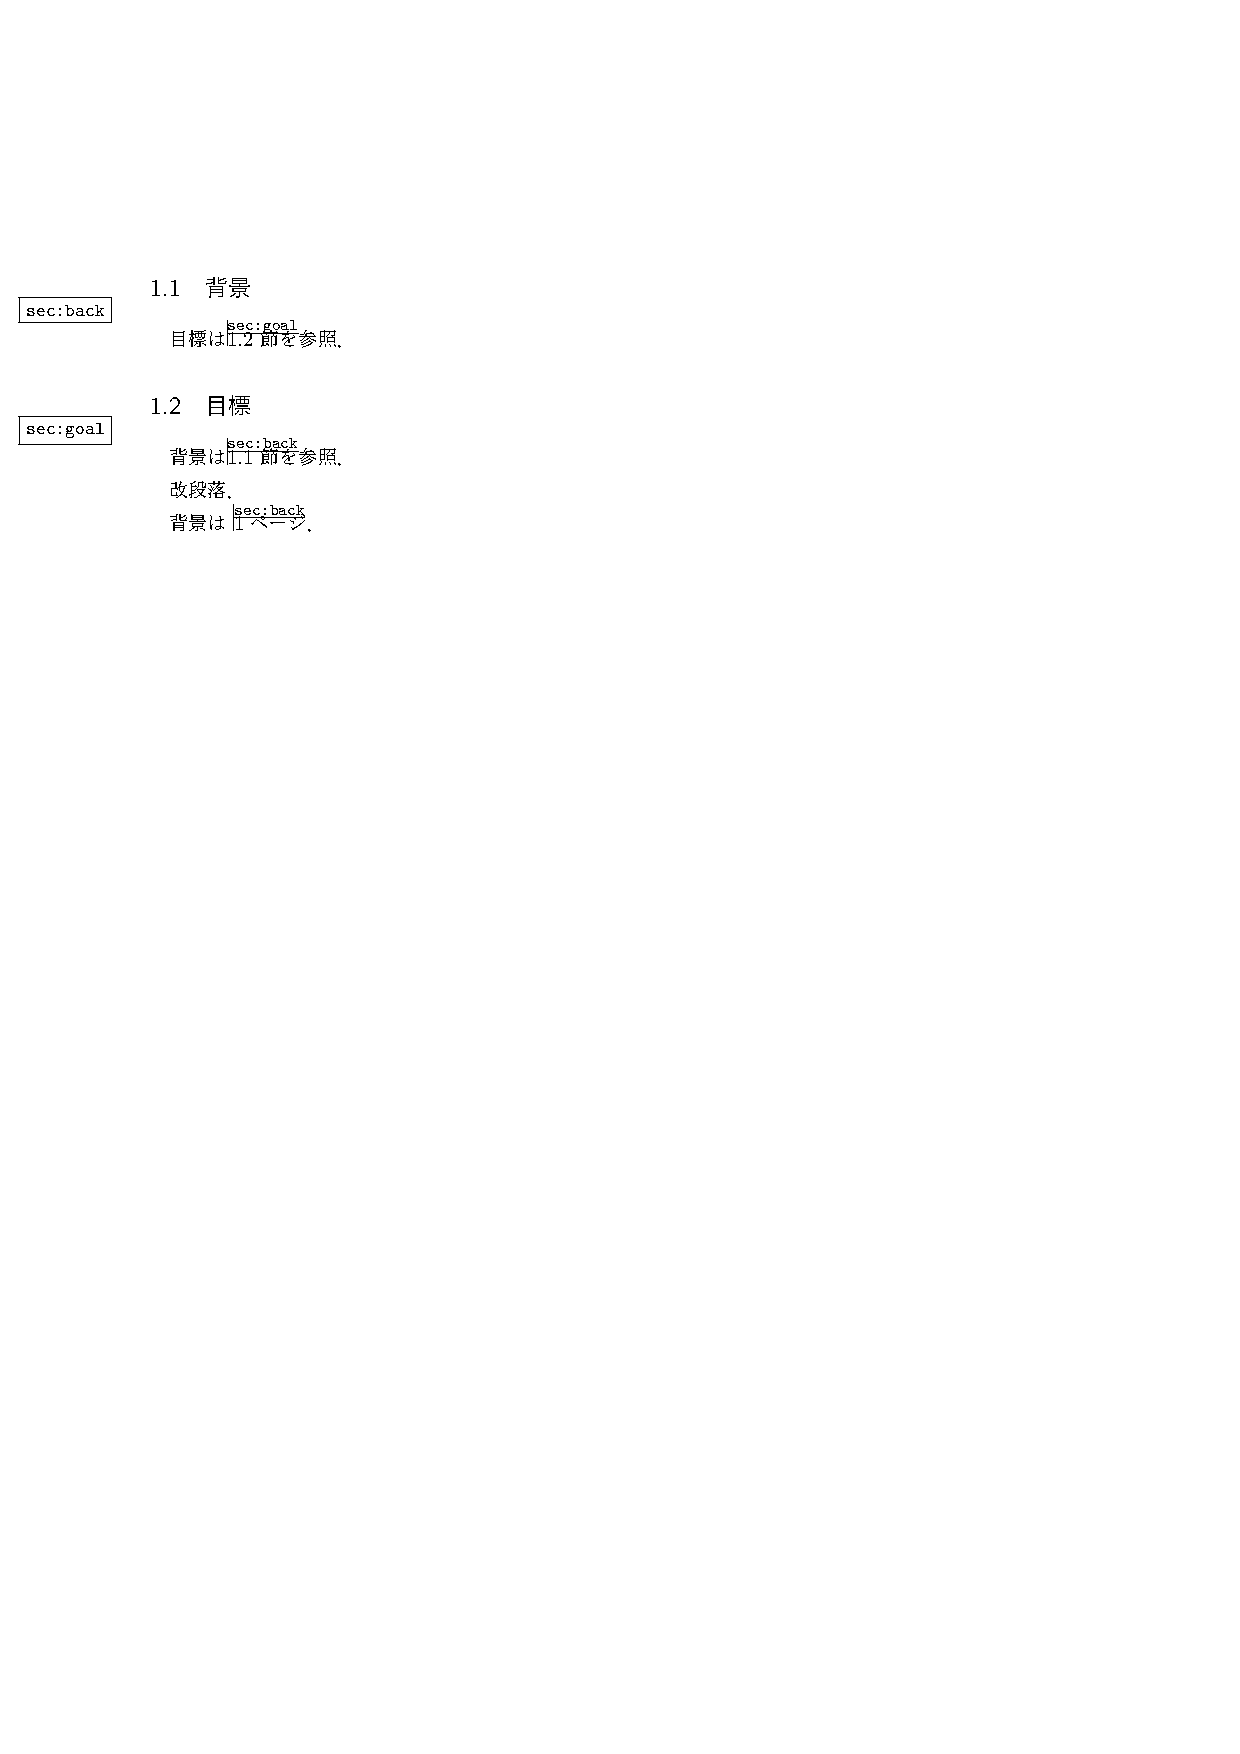
\includegraphics{showkeys} 
\end{outonly}

\subsection{カウンタ}
章見出しやページには通し番号が振られています.
これらは\K{\LaTeX カウンタ}によって制御
されています.カウンタはプログラミング言語で
言えばint型\pp{整数}の変数です.
%{\LaTeX}ではこ%
%\zindind{カウンタ}{レジスタ}%
%れを\K{カウンタレジスタ}
カウンタ変数の仕組みや制御の方法を少しは知っておいた
ほうが後々便利です.%この章では変数の基礎を説明します.

例えば\cls{jsbook}クラスで章\pp{\cmd{chpater}}の
下の階層の節\pp{\cmd{section}}用のカウンタを
新設するには \C{newcounter}命令を使って次のようにします.

\begin{intext}
\newcounter{section}[chpater]
\end{intext}

このようなカウンタの操作には
次の命令が使えます.\zindind{カウンタ}{の新設}%
\zindind{カウンタ}{の設定}%

\subsection{カウンタを新設する}
\begin{usage}
\newcounter{$\<カウンタ名>$}[$\<親カウンタ名>$]
\end{usage}

\subsection{カウンタの値を操作する}
\begin{usage}
\setcounter{$\<カウンタ名>$}{$\<整数値>$}% カウンタの値を設定する
\addtocounter{$\<カウンタ名>$}{$\<整数値>$}% カウンタに値を足す
\stepcounter{$\<カウンタ名>$}% カウンタの値を一つ増やす
\refstepcounter{$\<カウンタ名>$} % 相互参照が可能な \stepcounter
\end{usage}

\subsection{カウンタの値を参照する}
\begin{usage}
\value{$\<カウンタ名>$} % 値を表示・参照する
\end{usage}


\cmd{newcounter}でカウンタを新設します.
\cmd{setcounter}は数値を代入し,
\cmd{addtocounter}は数値を足し,
\cmd{stepcounter}はカウンタの値を
一つだけ増やします.\Cmd{refstepcounter}は
カウンタを後から参照できるようにラベルが
用意されます.\cmd{stepcounter}と \cmd{refstepcounter}
によって親カウンタが増えるとその子であるカウンタは
0にリセットされます.\cmd{value}はカウンタから
親カウンタの値や文字列などを取り除いた純粋な
カウンタの値が得られるコマンドです.

カウンタの表示形式を変更するものに以下があります.
\begin{usage}
\arabic   $\text{(1, 2, \ldots)}$
\roman    $\text{(i, ii, \ldots)}$
\Roman    $\text{({I}, {II}, \ldots)}$
\alph     $\text{({a}, {b}, \ldots, z)}$ (1〜26)
\Alph     $\text{({A}, {B}, \ldots, Z)}$ (1〜26)
\fnsymbol $\text{({*}, \textdagger, \ldots)}$ (1〜9)
\end{usage}

例えば節\pp{\cmd{section}}の見出し番号を
ローマ数字に変更するのであれば,節見出し用の
カウンタ\qu{\kount{section}}を次のように
再定義します.

\begin{intext}
\renewcommand{\thesection}{\Roman{section}}
\end{intext}

%%\begin{Prob}
%%以下のファイルをタイプセットし,その実行結果を吟味してください.
%
%\begin{intext}
%\documentclass{jsarticle}
%\renewcommand\thesection{\Alph{section}}
%\begin{document}
%\tableofcontents
%\section{序論}
%\subsection{構成}
%\end{document}
%\end{intext} 
%
%この結果から,\C{thesection} のみを変更するだけで十分かどうか
%検討してください.
%%\end{Prob}
